\documentclass[border=4pt]{standalone}
\usepackage{amsmath,amssymb}
\usepackage{tikz}
\usetikzlibrary{arrows.meta,shadows}
\begin{document}
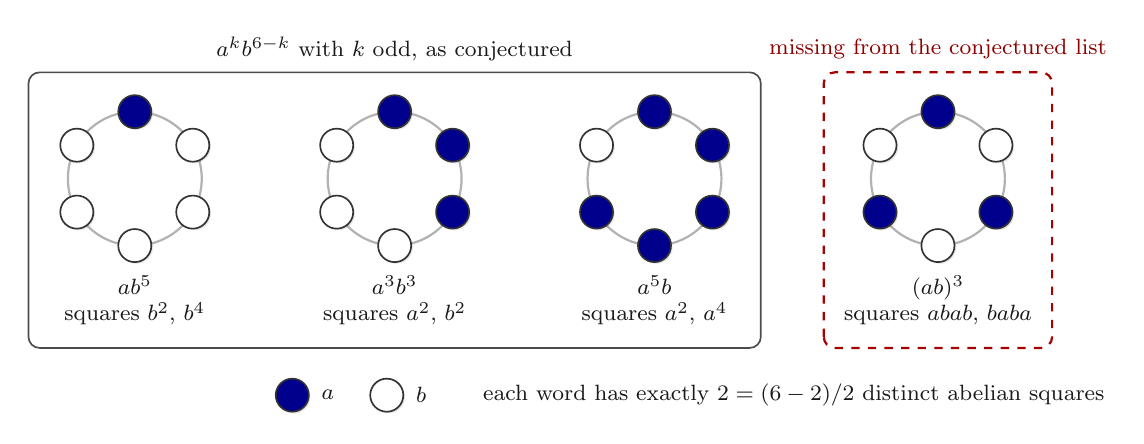
\begin{tikzpicture}[
  note/.style={font=\footnotesize,gray!20!black,align=center},
  bead/.style={circle,draw=black!80,line width=0.6pt,minimum size=4.2mm,inner sep=0pt,
               drop shadow={opacity=0.2,shadow xshift=0.6pt,shadow yshift=-0.6pt}},
  A/.style={bead,fill=blue!55!black},
  B/.style={bead,fill=white}]
  % a necklace of length 6 at (#1), letters #2 (a list of A/B), read clockwise from the top
  \newcommand{\necklace}[2]{
    \draw[gray!60,line width=0.8pt] (#1) circle (0.85);
    \foreach \t [count=\s from 0] in {#2} {
      \node[\t] at ($(#1)+({90-60*\s}:0.85)$) {};
    }
  }
  \usetikzlibrary{calc}
  \necklace{0,0}{A,B,B,B,B,B}
  \necklace{3.3,0}{A,A,A,B,B,B}
  \necklace{6.6,0}{A,A,A,A,A,B}
  \necklace{10.2,0}{A,B,A,B,A,B}
  \node[note] at (0,-1.55) {$ab^5$\\ squares $b^2$, $b^4$};
  \node[note] at (3.3,-1.55) {$a^3b^3$\\ squares $a^2$, $b^2$};
  \node[note] at (6.6,-1.55) {$a^5b$\\ squares $a^2$, $a^4$};
  \node[note] at (10.2,-1.55) {$(ab)^3$\\ squares $abab$, $baba$};
  \draw[red!65!black,rounded corners=4pt,line width=0.8pt,dashed] (8.75,-2.15) rectangle (11.65,1.35);
  \node[note,red!55!black] at (10.2,1.65) {missing from the conjectured list};
  \draw[gray!60!black,rounded corners=4pt,line width=0.6pt] (-1.35,-2.15) rectangle (7.95,1.35);
  \node[note] at (3.3,1.65) {$a^kb^{6-k}$ with $k$ odd, as conjectured};
  \node[bead,fill=blue!55!black] at (2.0,-2.75) {};
  \node[note,anchor=west] at (2.25,-2.75) {$a$};
  \node[bead,fill=white] at (3.2,-2.75) {};
  \node[note,anchor=west] at (3.45,-2.75) {$b$};
  \node[note,anchor=west] at (4.3,-2.75) {each word has exactly $2=(6-2)/2$ distinct abelian squares};
\end{tikzpicture}
\end{document}
